%Theory --- important this is clear as possible
% first trial includes a lot of figures as it makes it clearer to me

\chapter{Theory}

\section{Introduction to Theory}
An overview of the relevant theoretical concepts is included in this chapter. To most effectively discuss this the key terms as used here are first outlined. These terms include citizen science, stakeholders, local knowledge, vulnerability, place, and awareness and are used through the rest of the thesis. Resilience is here considered as the outcome from the process of the interacting systems which are clumped for ease of understanding into three categories of natural systems, technological systems and social systems. By expanding upon \cite{cutter_place-based_2008} to answer the needs highlighted in \cite{rasanen_conceptualizing_2020} this thesis presents projected resilience of place as the theoretical framework. 


\section{Key Terms}

\subsection{Citizen Science}
Citizen science can take many varied forms, but the common factor is the involvement of volunteers. People who chose to use their time to assist in science who are not paid for their time \cite{pocock_choosing_2014}. Considering \cite{tweddle_guide_2012} the participation of volunteers was deemed critical for this project and will assist in the overall aims. This is because the data required would not be accessible using other techniques and the research was designed to improve the awareness of sea level extremes in Trondheim. The volunteers, who will henceforth be referred to as subjects, contributions were respected and the impact of their time by the research was minimised. After this project submission the results will be published in an accessible form for those subjects who are interested. This is inline with the guidelines for citizen science set out by \cite{tweddle_guide_2012} The data management plan and ethics guidance were created inline with \cite{nesh_guidelines_2022} and \cite{nsd_norsk_nodate}.


\subsection{Stakeholders}
The stakeholders primarily considered during this project are the people who live commute or work in coastal Trondheim. This was decided using \cite{reed_stakeholder_nodate} as a back up for a very basic stakeholder analysis. Other stakeholders considered are people with attachment to the research sites as well as well as planners and policy makers. Creating a full understanding prior to research of who was a stakeholder was not a priority as the primary research method relies upon stakeholders to self identify by choosing to take part in this research. However, targeting of subjects utilising the decided upon stakeholders was done. 

\paragraph{}
The stakeholders identity is a key part of the research. The nature of stakeholder participation during this project was limited to communication and consultation according to Rowe and Frower 2000 in \cite{reed_stakeholder_nodate}. How these stakeholders are categorised was predominately top down as community membership of certain groups were targeted with the ability to identify as these groups during the survey \cite{reed_stakeholder_nodate}. However, there was also bottom up stakeholder identification as subjects could write in which groups they felt part of, beyond those decided on during the project design\cite{reed_stakeholder_nodate}. Stakeholder theory is not one of the lenses in which these results are analysed, however an understanding of what and who the stakeholders are in the changing impacts of sea level extremes in Trondheim was essential to allow the assessment of local knowledge and awareness. 

\subsection{Local Knowledge}

Local knowledge is considered here as place-based competence, information and resources \cite{setten_we_2019}. Over time local knowledge is co-produced and maintained by a range of experts by locally situated and beyond the areas boundaries. The quote "We draw on what we know anyway" from \cite{setten_we_2019} is a very succinct conceptualisation of local knowledge within the context of disaster risk management.

\begin{figure}[h]
    \centering
    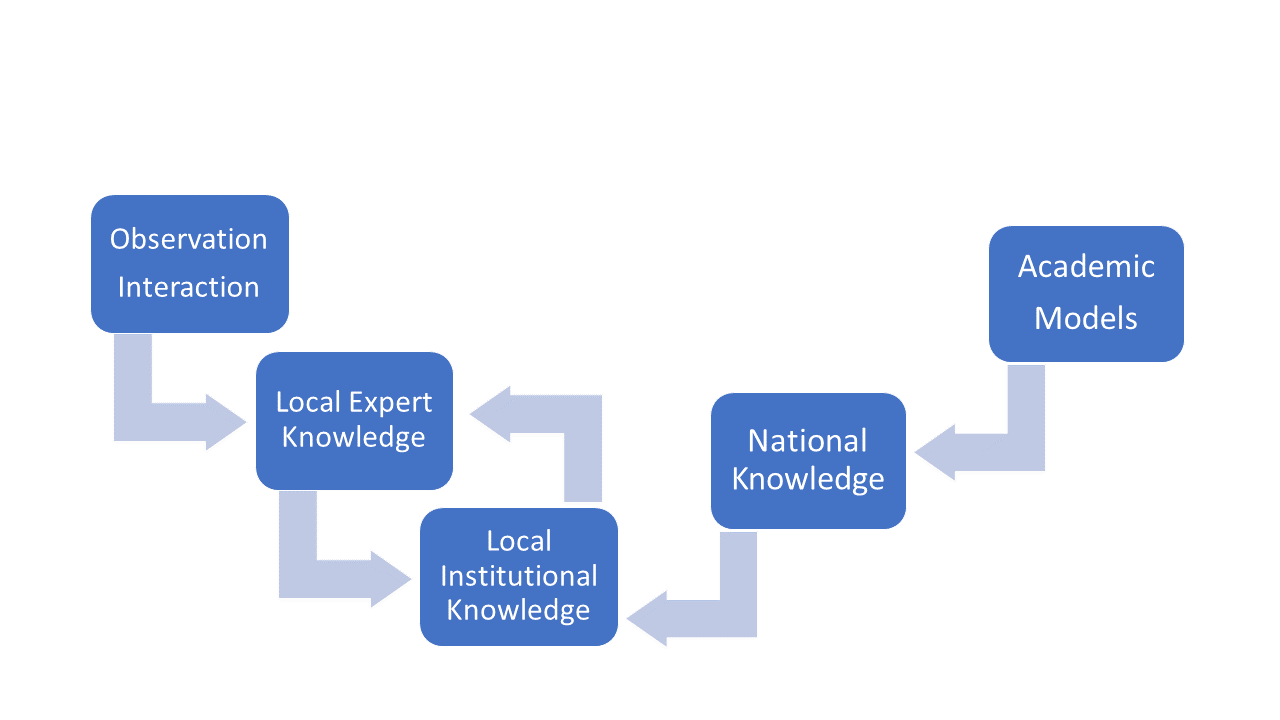
\includegraphics[width=1\textwidth]{fig_theory/local knowledge accumulation.png}
    \caption{Figure Local Knowledge Production. Created using the information stream outlined in \cite{setten_we_2019} and \cite{rod_integrated_2012} Local expert knowledge is produced by observation and interactions, often in the local sphere. Local expert Knowledge co-produces with local institutional knowledge each feeding into the other. Academic models helps produce national knowledge which in turn feeds into local institutional knowledge. Increasing the interplay between local expert knowledge and local institutional knowledge can increase resilience \cite{setten_we_2019}}
    \label{fig:local_knowledge}
\end{figure}


As can be seen in figure** above Local Expert knowledge is created as many may assume from local observations and local interactions. Yet, local expert knowledge also is created from local institutional knowledge. This local institutional knowledge is in turn co-produced by local expert knowledge. In this case the local expert knowledge is often considered more informal than the formalised local institutional knowledge, but does not need to be limited to this.  Academic models and national knowledge do feed into local expert knowledge and local institutional knowledge. Yet, their has been highlighted that particularly for disaster risk management the local institutional and expert knowledge doesn't always feedback to these other producers of knowledge\cite{rod_integrated_2012}. The questions about the alignment between local knowledge and academic models of the changing sea level extremes influenced the creation of this project. 

\paragraph{}

Local knowledge is often highlighted as a key facet of community resilience \cite{setten_we_2019}. With the assumption being the higher levels of local knowledge particularly higher levels of awareness about natural systems and natural hazards increases community resilience.  How local knowledge interacts with community resilience and where this belongs in a place-based conceptualisation of resilience is discussed in the social systems of resilience section below. Awareness of local risk is here considered as a facet of local knowledge.  

 
%memory vs awareness vs knowledge 
 
\subsection{Vulnerability}
Vulnerability of a place is impacted by many broad influences including Local Knowledge 
Vulnerability – Lujala / Lein / Setten 



\subsection{Place and Space-time} 
To understand resilience we must ask resilience: for whom; of what; to what; of where; how and when \cite{cutter_community_2020}, \cite{moser_turbulent_2019}. Resilience is temporally and spatially dynamic \cite{cutter_community_2020}. Hence a basic description of what is meant here by space, time and place is necessary. The conceptualisation used here is inline with \cite{massey_for_2005}, where space is the dimension of simultaneity and is part of space-time. In this view space is considered as the dimension of things being and importantly occurring at the same time. In contrast time is considered as things occurring one after the other. This conceptualisation of space-time is relevant for private, public and even virtual spaces and gives room for the social networks that operate within these spaces \cite{massey_for_2005} \cite{allen_rethinking_1998}.

\paragraph{}
The four chosen research places are created upon a combination of public and private space. The majority of the edge of the water in Norway can be considered public space, but but there is also space allocated to specific groups which can create feelings of in-place vs out-of-place. Place is considered as an assemblage of traces. These traces range from the historical and global to the local and present and it is these combinations of traces which combine to make these places \cite{anderson_understanding_2015} \cite{massey_for_2005}. As well as explicit group membership the traces of place influence who can feel in-place and what is culturally and legally allowable uses of the places \cite{anderson_understanding_2015}. The four research sites include a wide demographic users of who can be considered in-place, but the power relationships and the in-place members affect the resilience of the location. 

\subsection{Awareness}
To understand the present resilience of a place requires an understanding of the awareness of the people who interact with and define the place. An individual’s ability to rank their level of awareness about a subject is a long investigated and debated topic *ref*. It is generally preferable to allow them to display their level of awareness rather than ask them on a sliding scale how aware they are. This is especially important when trying to explore knowledge which may have previously been seen as lesser.

\paragraph{}
To determine awareness level five questions were set in the survey used. These questions were designed to be simple and quick to answer in a format which would allow the author to analyse awareness about sea level extremes in the present and future along with general knowledge of the sea. Awareness about tide level, current risk of storm surges, past resilience to storm surges and future resilience to storm surges was investigated. Further information of how different question techniques and formats were trialled, and the influence of the decided questions format can be found in the Discussion section.

\begin{figure}[h]
    \centering
    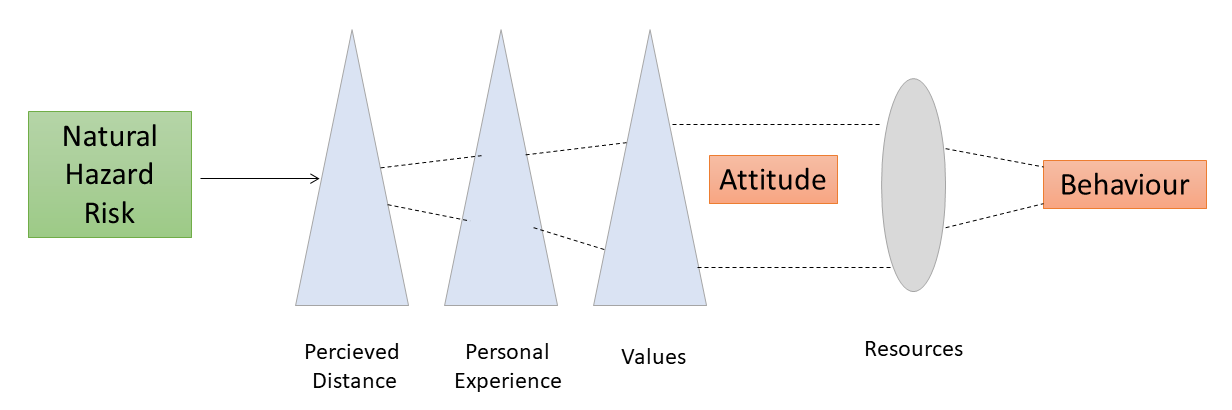
\includegraphics[width=1\textwidth]{fig_theory/awareness lujala and whitmarsh.png}
     \caption{Awareness of Natural Hazard Risk to behaviour pipeline based of \cite{lujala_climate_2015} and \cite{whitmarsh_are_2008} The awareness of Natural Hazard risk is filtered through perceived distance, then personal experience and then values before this interaction creates attitude. This attitude to the information about natural hazard risk is then filtered through the lend of resources before it creates behaviour.}
    \label{fig:my_awareness}
\end{figure}

Resilience is impacted by the behaviour of those who are potentially impacted by the potential hazard. Awareness is influenced by many factors. Figure 4.2 Awareness of Natural Hazard Risk to Behaviour pipeline is based on \cite{whitmarsh_are_2008} and \cite{lujala_climate_2015} . Where the green box labelled "Natural Hazard Risk" is the awareness of the individual about the risk. The three triangles are the prisms of "perceived distance", "personal experience" and "values" which have a significant impact on how this awareness is manifested as attitude to the natural hazard risk. This "attitude" is then put through the lens of "resources" before influencing the behaviour of the individual. 
\paragraph{}
Of course people's information in, to thought, to behaviour process are much more complicated than the visualisation above, but it is helpful to considered these prisms and lens when attempting to understand why individuals behave as they do. There is assumptions that those with higher levels of awareness about risks are more likely to have certain attitudes and in turn certain behaviours, but this is not always the case. \cite{lujala_climate_2015}  Awareness of the changing tides and risk of storm surges is considered here as an aspect of local knowledge and is one of the key factors investigated to determine the resilience of Trondheim to sea level extremes. 

\section{Theories Used}


\section{Theories of Resilience }

There are many theories on resilience and the term has many varied and wide conceptualisations. \cite{moser_turbulent_2019} highlights the recent increase in this term and discusses how different fields use the term resilience. Particularly the increase of the use in response to tragedy, especially tragedy associated with large uncontained systems. The climate is one such system and the political difficulty of discussing the climate crisis has led many politicians to instead focus on resilience building. 
\paragraph{}

This caused the term resilience to broaden to include a normative and trans-formative aspect.  This moves resilience away from a value that can be measured once, into a ongoing process which increases and decreases over time. The path of this needs to be understood, to prove increases in resilience as required by UN SDGs 11 and 13. Building resilience is often assumed to always be a desired outcome and is often raised in the response to disaster and especially tragedy \cite{moser_turbulent_2019}. This newer conceptualisation of resilience allows for greater focus on the integration of local knowledge, but this facet is not always included \cite{moser_turbulent_2019}.
\paragraph{}


\cite{cutter_place-based_2008} introduced the Determination of Resilience of Place. This was based on previous work on vulnerability and hazards of place \cite{cutter_vulnerability_1996}. Here vulnerability was labelled as the inherent qualities of the systems which create the potential for harm.
In contrast resilience is the ability to respond and recover which was inherently place based. However \cite{cutter_community_2020} moved away from place based resilience to focus on community resilience. Here resilience was considered as dynamic and dependent on three changing systems: natural, social and technological. Present resilience does not define future resilience, but it does influence it. So resilience be it place based or community resilience could only be measured post disaster. Both of these understandings of resilience were deemed vital to an overall view of resilience.
\paragraph{}

However \cite{rasanen_conceptualizing_2020} shows the limitations of place-based metric for measuring community resilience. \cite{rasanen_conceptualizing_2020} highlights the need for an alternative metric which can include community resilience and local knowledge but which can be repeatedly measured and viewed from a place-based conception of resilience. This is especially vital as in Norway the most common conceptualisation of community within national government, municipalities and individuals is place based \cite{rasanen_conceptualizing_2020}. To solve this issue the concept of projected resilience of place is put forward. 




\section{Projecting Resilience of Place} 
Resilience is here considered as the ability to return to normality as quickly as possible after an event, this is in line with \cite{cutter_place-based_2008}. Resilience is dynamic and the current levels of resilience do not define the future resilience, but they do have significant influence. Hence understanding of the current systems which create resilience and how they are changing can let us project resilience \cite{cutter_community_2020}. The view of resilience here incorporates many of \cite{moser_turbulent_2019} ideas about resilience -  that it can be a system trait, an outcome or a process. It considers projected resilience as a projected outcome, which is determined from systems. 

\cite{cutter_place-based_2008} and \cite{cutter_community_2020} discuss resilience in reference to disaster rather than event. Moving from measuring resilience post a disaster to projected resilience requires a consideration of the word disaster. Sea Level Extremes can cause disaster, but this is not necessarily the case. A sea level extreme thus can be viewed as a possible disaster which is referred to here as an event. 

An event is a potential disaster in which the systems absorbed the impacts in such a manner that normality was not lost. In terms of sea level extremes the daily tide flow is not a disaster as it in absorbed by the system and the systems cope to prevent this event from becoming a disaster. The sensitivity of the system is very rarely breached by the high tide in Trondheim. This distinction of events and disasters may be obvious for events which occur twice a day, but as extreme weather events become the norm due to the changing climate in an idealised set up what was once a potential disaster will now simply be an event. 

\begin{figure}[h!]
    \centering
    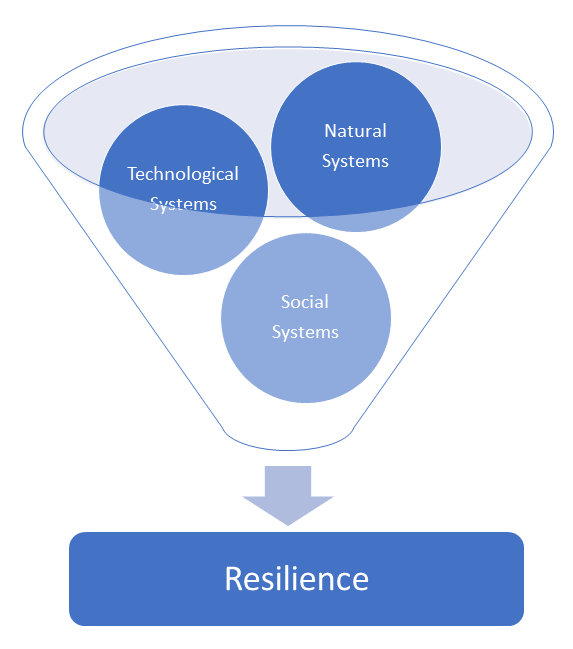
\includegraphics[width=0.5\textwidth]{fig_theory/resilience model .png}
    \caption{Model of Projected Resilience and the systems involved in its creation. The interplay of technological systems, social systems and natural systems creates resilience. }
    \label{fig:projected_resilience}
\end{figure}
wordssss

Projected resilience takes on the systems as laid out by \cite{cutter_community_2020}, but places community resilience under social systems. To allow for greater understanding between academic, policy makers and "layperson" due to the standard conceptualisation of community as placed based as highlighted by \cite{rasanen_conceptualizing_2020}. This is also to allow for an easier determination of resilience so it can be repeatedly measured, without loosing the aspects of community resilience or local knowledge. This risk is highlighted by \cite{rasanen_conceptualizing_2020}. The three systems of resilience as shown in figure 4.3 above are discussed individually in the sections below.

\section{Systems of Resilience }

\subsection{Social Systems impacting Resilience}
community resilience as key aspect of social systems
local knowledge is part of that

to determine social systems resilience of specific risk need to understand ......... and the awareness to the risk. 

\begin{figure}[h]
    \centering
    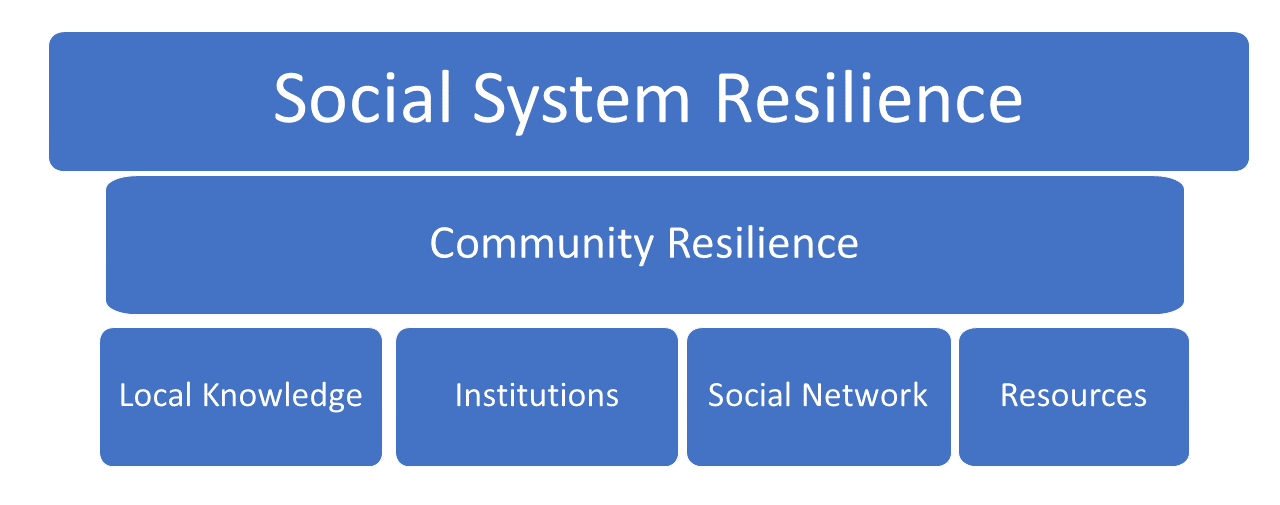
\includegraphics[width=1\textwidth]{fig_theory/social system hierarchy.png}
    \caption{Relationship between Community Resilience and Social System Resilience. Resources, social network, institutions and local knowledge are all important factors of Community Resilience. Within this text community resilience is considered as a major facet of social system resilience. Social system resilience is the overaching idea which is situated above community resilience.}
    \label{fig:social_resilience}
\end{figure}
\paragraph{}


words words words
\begin{figure} [h]
    \centering
    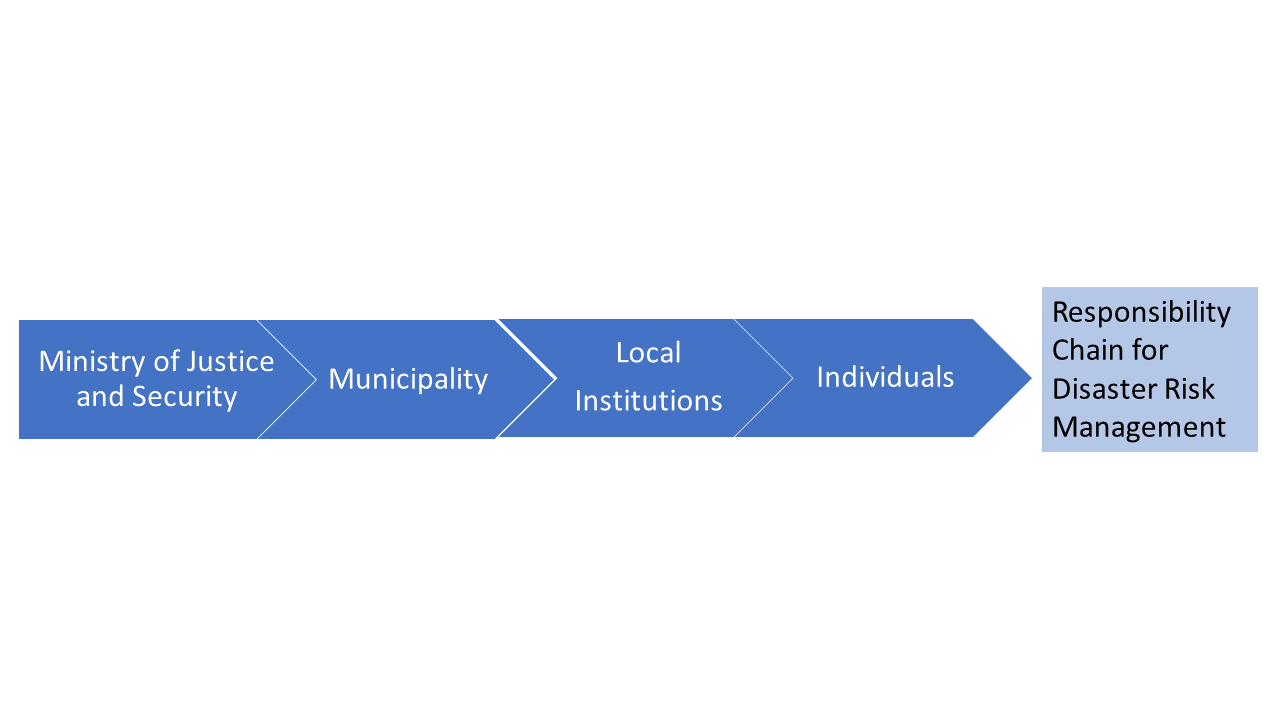
\includegraphics[width=1\textwidth]{fig_theory/responsibility drm.png}
    \caption{Responsibility Hierarchy for Disaster Risk Management in Norway. The ministry of Justice and Security has the overall responsibility for disaster risk management in Norway. This ministry issues responsibility to the municipality, who in turn issues responsibility for preparation of disasters to both individuals and local institutions.}
    \label{fig:drm_responsibility}
\end{figure}
\paragraph{}

\subsection{Technological Systems}
%altered coastlines
%observation - watching of coastlines - e.g. person falling in notice scheme in trondheim
%infrastructure 
%models of coastlines



\subsection{Natural Systems }
When discussing sea levels in this thesis it will always be done in reference to NN2000. Sea Level extremes are the extreme to which the sea reaches in height and area. The most common sea level extreme is the spring tide. Sea Level extremes in Trondheim are the combination of the impact of waves, the height of the sea, tides, storm surges and land movement \cite{hanssen-bauer_climate_2017}, as can be seen in figure ** . In the research site Nidelva there is also the added impact of the level of the river. There is generally high levels of uncertainty in the projection of storm surges \cite{nilsen_sealevelchangefornorway_nodate}. Changing wind patterns are hard to predict \cite{rod_three_2015} and storm surges and the sea level extremes they cause are dependent on the wind. Storm surges - called stromflo in Norwegian -  occur due to the weather conditions including strong on shore winds and low air pressure. \cite{hanssen_saksframlegg_2013'}

\paragraph{}

Reference will be made to the 20 year storm surge throughout this thesis, which is the projected recurrence interval of a storm surge of a particular height. Meaning that that there is a 5 percent chance of it happening each year as this storm surge on average occurs once every 20 years, meaning \cite{hanssen_saksframlegg_2013}. . However the recurrence of this storm surge height could occur at much shorter intervals. This is one of the major impacts of climate change, known as global weirding, where unusually events occur more often. The calculations for sea level extremes in this report mainly utilise the IPCCs fifth assessment report emission scenario RCP 8.5, which is the emission projection for business as normal \cite{hanssen-bauer_climate_2017}, due to the uncertainty of the calculations and to avoid underestimating the vulnerability and overestimating resilience.  




\begin{figure}[h!]
    \centering
    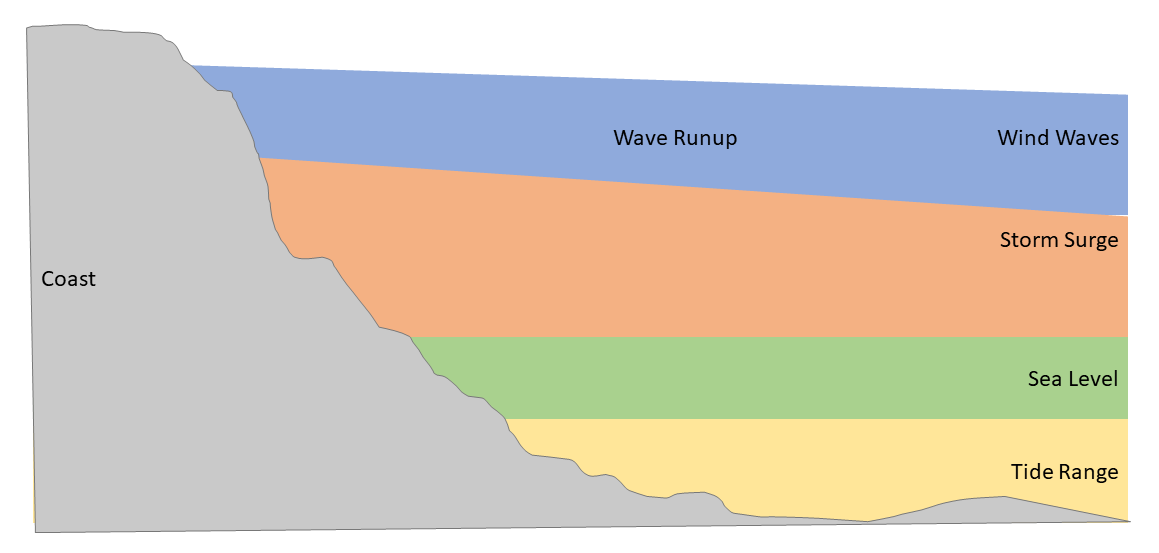
\includegraphics[width=1\textwidth]{fig_theory/sea level extremes.png}
    \caption{The various aspects which combine to create extreme sea levels: Tide Range, Sea Level, Storm Surge, Waves due to the wind, Waves due to the run-up onto the coast}
    \label{fig:my_label}
\end{figure}

Figure 4.6 above shows the natural aspects which combine to create sea level extremes. Which factor is most important will be different for each location, however for the Trondheim the current largest change in risk is storm surges. 

The impact due to waves which may change with the changing climate is predicted to cap out at 2m within the time frame considered here. The Safety class 1 of the building regulations TEK10/TEK17 as used since 2016, corresponds with the 20 year storm surge \cite{tides_high_2022}. The temporal variability and land use characteristics could be considered in an analyse of the natural systems resilience to storm surges. However these factors appear to have minimal impact in urban and semi-urban environments \cite{hoffken_effects_2020}

\section{Sustainability vs Resilience}

Sustainability is a term with increasing use and interest over the last decades. There are many similarities between this concept and the concept of resilience. However the dynamism of the term resilience and its lack of solidified political meaning puts it in favour, particularly with groups often self excluded from discussions on sustainability \cite{moser_turbulent_2019}. This politicisation of the term has benefits and negatives, but risks changing the meaning.
\paragraph{}

While \cite{moser_turbulent_2019} highlights the increasing use of the term resilience to mean an organizing strategy for handling complex systems with high levels of uncertainty, especially in political spheres. This understanding of resilience did not seem the most appropriate for sea level extremes in Trondheim. In part because the high levels of acceptability of the climate crisis both in the local population and in the political spheres, locally, regionally and nationally. 

Within the political context of Trondheim neither climate change nor sustainability are excluded terms. Keeping these terms distinct from resilience, allows for a more nuanced discussion.







